\chapter{Evaluation} 

\section{Controlled Movements}
\label{sec:controlled_movements}

% Comparison deadreckoning accuracy of battery powered robot with solar powered robot

% Try at least one more supercapacitor: 10mF
% Study reducing the frequency of power interrupts ie smaller energy buffer.
% How does this effect the accuracy of locomotion?
% Can the frequency of power interrupts be related to the 

% Video of robot movement

In this section the accuracy of movement of the battery-less robot and its battery powered counterpart will be compared.

\subsection{Experimental setup}

To be able to compare the accuracy of the robot while it is exposed to increasingly smaller power cycles, a variety of movements is recorded using a overhead camera.
A camera stand with a Nikkon D610 DSLR camera is positioned on a tabletop and in the camera's view the corners of a square of 80$\times$80\,cm are indicated with a black marker, see Figure \ref{fig:movement_setup}.
This square is later used as a reference to convert the robots movement from pixels to cm.
Three different movements are compared, while the robot is moving straight movement of 75\,cm, a circle with radius of 30\,cm and a square of 50$\times$50\,cm.

\begin{figure}
	\centering
	\begin{subfigure}[b]{0.45\textwidth}
		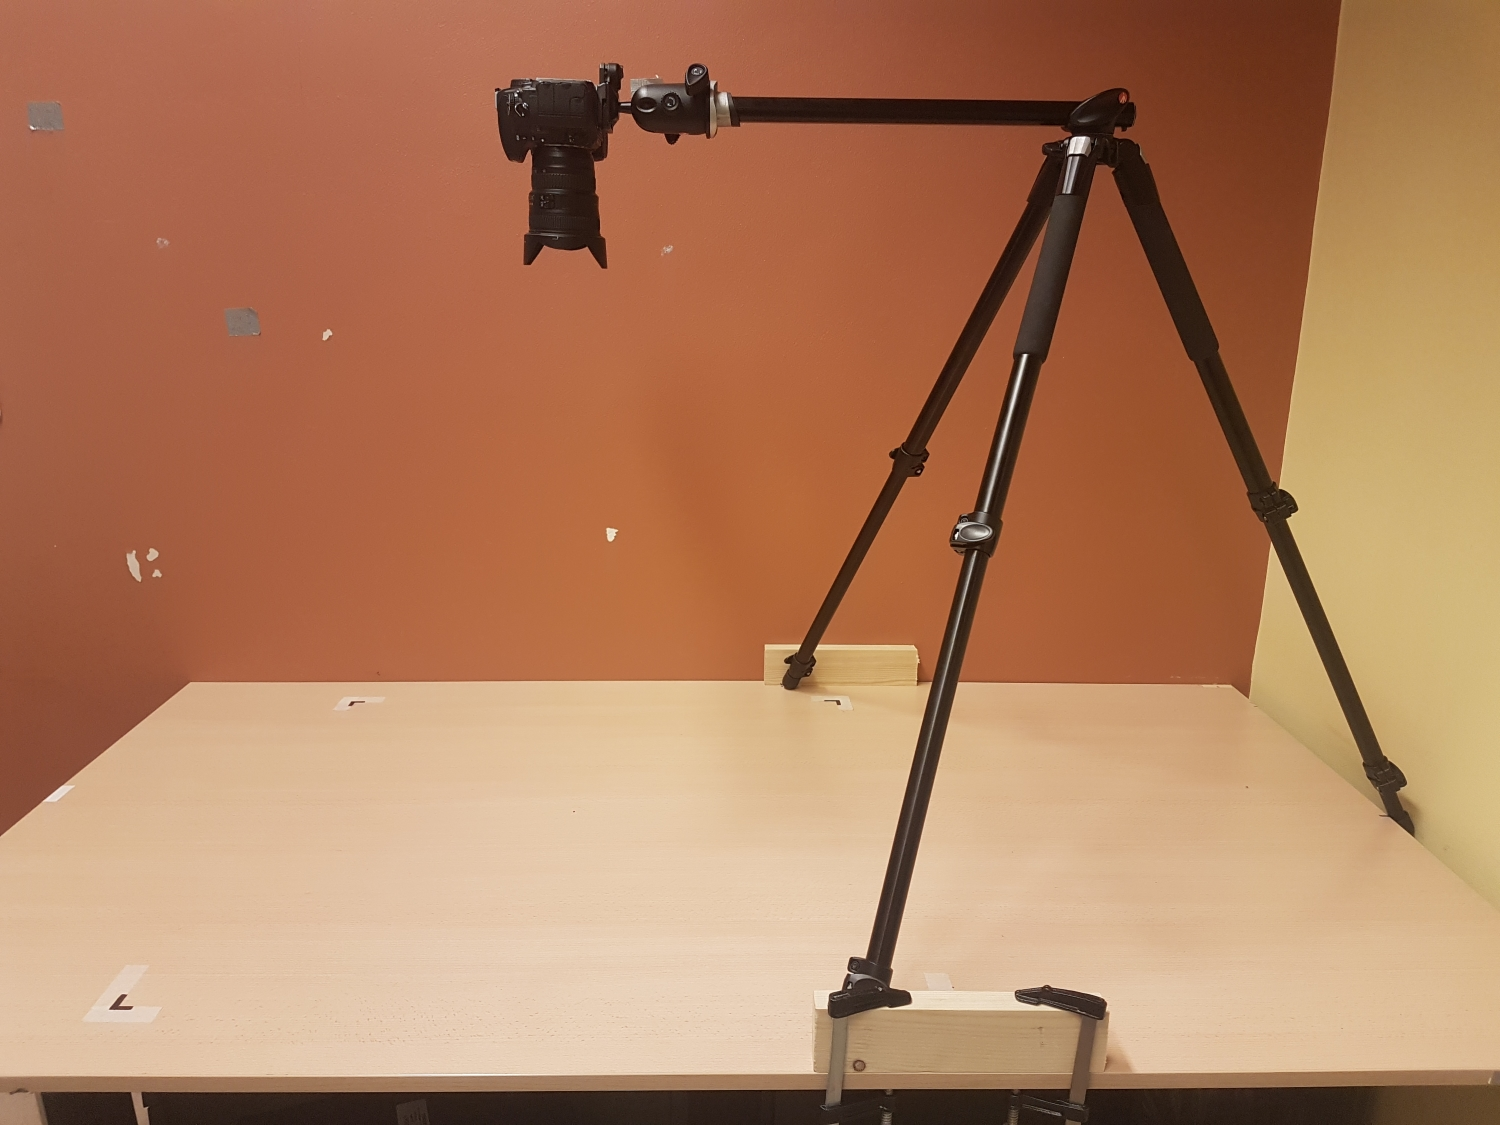
\includegraphics[width=\textwidth]{pics/movement_setup.jpg}
		\caption{Camera setup}
		\label{fig:movement_setup}
	\end{subfigure}
	\quad
	\begin{subfigure}[b]{0.45\textwidth}
		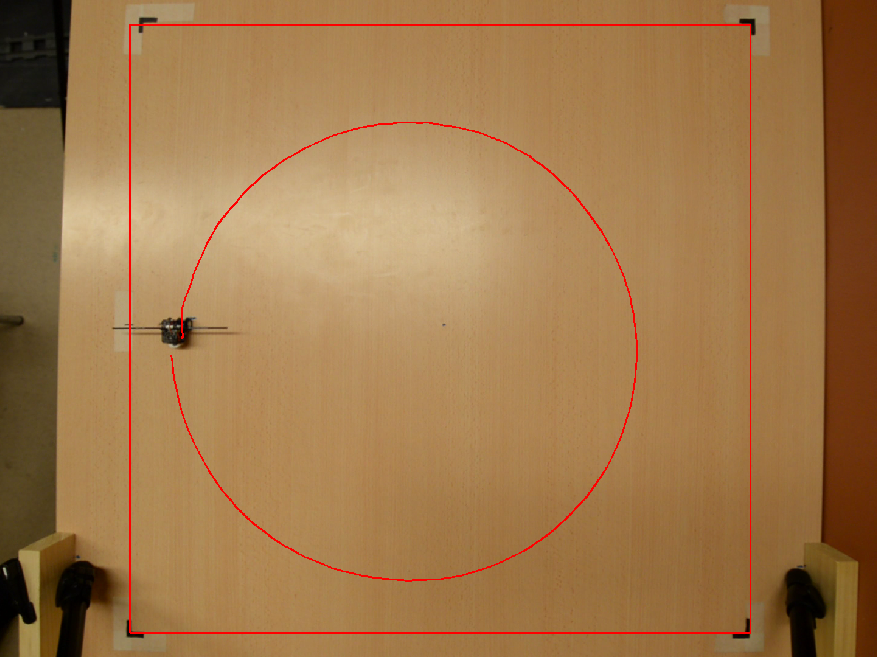
\includegraphics[width=\textwidth]{pics/movement_example.png}
		\caption{Tracking with OpenCV}
		\label{fig:movement_example}
	\end{subfigure}
	\caption{Experimental setup to record the robots movement}
\end{figure}

\subsubsection{Tracking the Movement}

%The robot is programmed to preform the movement at a desired PWM target ie at a specified speed, and optional power interrupt period.
Before the robot executes the movement a green led is enabled on top of the robot.
This green dot will be the reference point that the tracking software will try to follow.
The camera is used to record the movement which then is analyzed using Python and OpenCV 3.2.
An example of a tracked movement can be seen in Figure \ref{fig:movement_example}.

\subsubsection{Target Speed Setting}
To evaluate the influence of speed each movement is executed at three different speed target settings: 40\%, 65\% and 90\% of the maximum duty cycle.
Choosing a target higher than 90\% is undesired while the controller needs some room to adjust the speed up and down to control the robots heading.

\subsubsection{Power Interrupts}

To evaluate different power cycle periods without changing the capacitor size or the minimum and maximum voltage thresholds set using resistors, power interrupts are generated artificially.
During the experiment the robot will be powered from a battery and power interrupts, i.e the capacitor running out of energy are created artificially using a timer that resets the MCU.
The MSP430FR5969 has the functionality to enable a brownout reset trough software which is used to simulate the event of the supply voltage dropping below the required operating voltage~\cite{msp430fr_family_guide_2017}.
A timer is used to generate the power interrupt after a predefined period.

\subsubsection{Power Interrupt Period}

With the selected capacitor of 22\,mF the robot can operate around 1 second. 
Choosing a period of 0.25\,s showed uncontrolled behavior, while the robots control loop was not able to stabilize the movement before a power interrupt occurs.
To find the minimal power interrupt period that is required to control the robot, the robot is programmed to preform a four second straight movement.
The movement is recorded for each target speed and the power interrupt periods of 0.4\,s, 0.3\,s and 0.2\,s are evaluated.

The results in Figure \ref{fig:decreasing_power_period} show that a interrupt period of 0.2\,s results in uncontrolled behavior, while the robot drifts to the side of the weakest motor.
Increasing the target speed shows that also a higher interrupt period period is required to control the movement. 
The power interrupt periods evaluated in this experiment were set to values above and equal to 0.5\,s: 1.25\,s, 1\,s, 0.75\,s and 0.5\,s.


\begin{figure}
	\begin{subfigure}[b]{0.32\textwidth}
		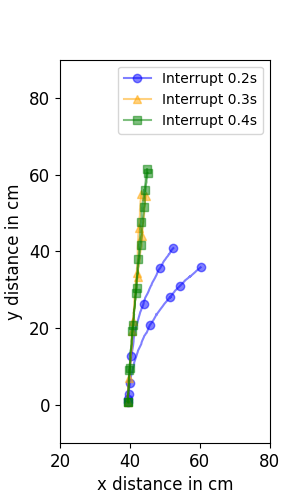
\includegraphics[width=\textwidth]{pics/figure_40.png}
		\caption{Target 40\%}
		\label{fig:target_40}
	\end{subfigure}
	\begin{subfigure}[b]{0.32\textwidth}
		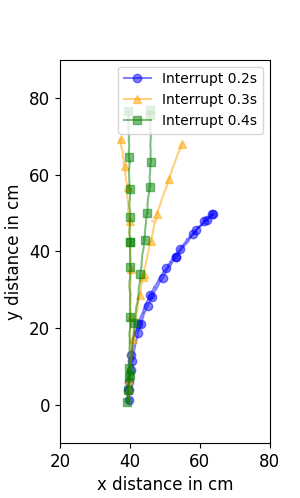
\includegraphics[width=\textwidth]{pics/figure_65.png}
		\caption{Target 65\%}
		\label{fig:target_65}
	\end{subfigure}
	\begin{subfigure}[b]{0.32\textwidth}
		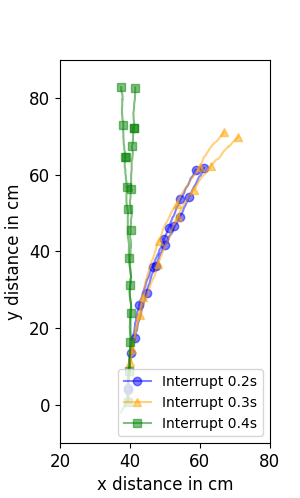
\includegraphics[width=\textwidth]{pics/figure_90.png}
		\caption{Target 90\%}
		\label{fig:target_90}
	\end{subfigure}
	\caption{Accuracy of movement with decreasing the power interrupt period.}
	\label{fig:decreasing_power_period}
\end{figure}

\subsubsection{Velocity Calibration}
Another thing that can be observed from the results in Figure \ref{fig:decreasing_power_period}, is that the distance covered by the robot deceases by deceasing the target and/or power interrupt period.
Without any sensors or external feedback that can determine the robots speed, it is difficult to determine the distance that the robot has traveled.
The average speed is estimated for each speed target and power interrupt period.
This is achieved by first determining the time that the robot requires to move approximately 150\,cm for each target without power interrupts.
When the robot experiences power interrupts the average velocity of an active period becomes lower due to frequent acceleration from a standstill.
With power interrupts the runtime is increased to make the robot travel roughly the same distance.
Finally, the average of five complete movement measurements is computed and divided by the commanded runtime of the robot to acquire an average speed for each combination, as seen from Table \ref{tab:val_calib}.


\begin{table}[t]
	\centering
	\small
	\caption{Calibrated velocity}
	\label{tab:val_calib}
	\begin{tabular}{|l|l||l|l|l|l|l|l|}
		\hline
		Target (\%) & & No int & Solar & 1.25\,s & 1.0\,s & 0.75\,s & 0.5\,s \\
		\hline \hline
		 40 & cm/s & 18.9 & 16.0 & 18.2 & 18.0 & 17.1 & 15.9 \\
	     65 & cm/s & 24.0 & 20.8 & 22.2 & 21.3 & 20.8 & 18.8 \\
		 90 & cm/s & 28.8 & 23.3 & 26.4 & 25.7 & 24.5 & 22.7 \\
		\hline
	\end{tabular}
\end{table}

\subsection{Straight Movements}

Using the calibrated velocities and selected power interrupt periods, the robot is commanded to preform a straight movement of 75\,cm.
Each combination is recorded multiple times and the motion data is extracted from the video using Python and OpenCV.
The results in Figure \ref{fig:straight_movements} show that the robot roughly moves the commanded 75\,cm.

\begin{figure}
	\centering
	\begin{subfigure}[b]{0.32\textwidth}
		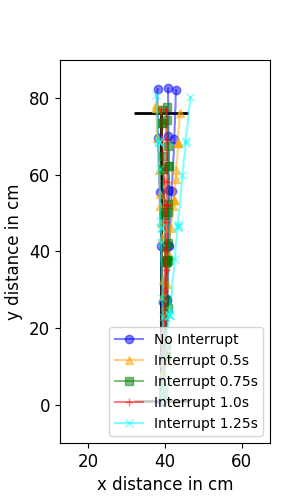
\includegraphics[width=\textwidth]{pics/straight_40.png}
		\caption{Target 40\%}
		\label{fig:stra_exp1}
	\end{subfigure}
	\begin{subfigure}[b]{0.32\textwidth}
		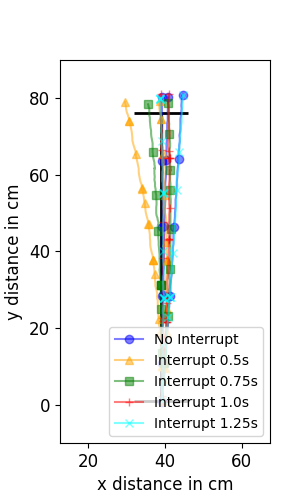
\includegraphics[width=\textwidth]{pics/straight_65.png}
		\caption{Target 65\%}
		\label{fig:stra_exp2}
	\end{subfigure}
	\begin{subfigure}[b]{0.32\textwidth}
		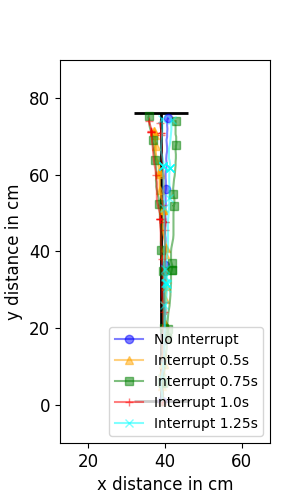
\includegraphics[width=\textwidth]{pics/straight_90.png}
		\caption{Target 90\%}
		\label{fig:stra_exp3}
	\end{subfigure}
	\caption{Straight movements, the black horizontal line shows the 75\,cm endpoint}
	\label{fig:straight_movements}
\end{figure}

\subsubsection{Movement Accuracy Metrics}
NO EXTERNAL FEEDBACK

Even though the robot is positioned carefully in the same start position, it is inevitable that the robot is positioned non-perpendicular to the reference frame of 80$\times$80\,cm, i.e. the robot will start moving on a angle.
Therefore 

\begin{itemize}
	\item average curvature of straight line movement

	\item for both straight and curved movements: length of the total movement and standard deviation in length of movement
\end{itemize}


\subsubsection{Straight Movement Results}

\begin{table}[t]
	\centering
	\caption{The Euclidean distance between the recorded data and a straight line between the begin and endpoint of the data.}
	\label{tab:straight_results}
	\begin{tabular}{|l|l||l|l|l|}
		\hline
		Target (\%) & Interrupt (s) & Max (cm) & Mean (cm) & Std (cm)\\
		\hline \hline
		\multirow{5}{*}{40} & No int & 0.86 & 0.36 & 0.16 \\
		& 1.25 & 0.67 & 0.34 & 0.12 \\
		& 1.00 & 1.35 & 0.56 & 0.27 \\
		& 0.75 & 1.04 & 0.60 & 0.27 \\
		& 0.50 & 0.86 & 0.44 & 0.22 \\
		\hline
		\multirow{5}{*}{65} & No int & 0.52 & 0.25 & 0.12 \\
		& 1.25 & 0.72 & 0.31 & 0.14 \\
		& 1.00 & 0.91 & 0.44 & 0.21 \\
		& 0.75 & 1.44 & 0.80 & 0.35 \\
		& 0.50 & 2.15 & 1.17 & 0.54 \\
		\hline
		\multirow{5}{*}{90} & No int & 0.54 & 0.28 & 0.13 \\
		& 1.25 & 0.90 & 0.42 & 0.17 \\
		& 1.00 & 1.76 & 0.95 & 0.42 \\
		& 0.75 & 1.88 & 0.88 & 0.37 \\
		& 0.50 & 2.18 & 1.09 & 0.61 \\
		\hline
	\end{tabular}
\end{table}

\subsection{Circular Movements Results}

The robot is commanded make a circle with radius of 30\,cm
\subsubsection{Movement Accuracy Metrics}



\begin{table}[t]
	\centering
	\caption{The mean and standard deviation of the Euclidean distance from the fitted circle.}
	\label{tab:circular_results}
	\begin{tabular}{|l|l||l|l|l|}
		\hline
		Target (\%) & Interrupt (s) & Radius (cm) & Mean (cm) & Std (cm)\\
		\hline \hline
		\multirow{5}{*}{40} & No int & 34 & 1.3 & 0.67 \\
		& 1.25 & 32 & 1.29 & 0.69 \\
		& 1.00 & 32 & 1.52 & 0.81 \\
		& 0.75 & 33 & 1.21 & 0.82 \\
		& 0.50 & 32 & 1.85 & 1.30 \\
		\hline
		\multirow{5}{*}{65} & No int & 34 & 1.2 & 0.67 \\
		& 1.25 & 32 & 1.01 & 0.57 \\
		& 1.00 & 32 & 1.42 & 0.92 \\
		& 0.75 & 33 & 1.11 & 0.73 \\
		& 0.50 & 32 & 0.79 & 0.34 \\
		\hline
		\multirow{5}{*}{90} & No int & 30 & 0.9 & 0.45 \\
		& 1.25 & 30 & 0.81 & 0.43 \\
		& 1.00 & 31 & 1.06 & 0.65 \\
		& 0.75 & 31 & 0.71 & 0.41 \\
		& 0.50 & 35 & 1.69 & 1.23 \\
		\hline
	\end{tabular}
\end{table}


\begin{figure}[h!]
	\centering
	\begin{subfigure}[b]{0.5\textwidth}
		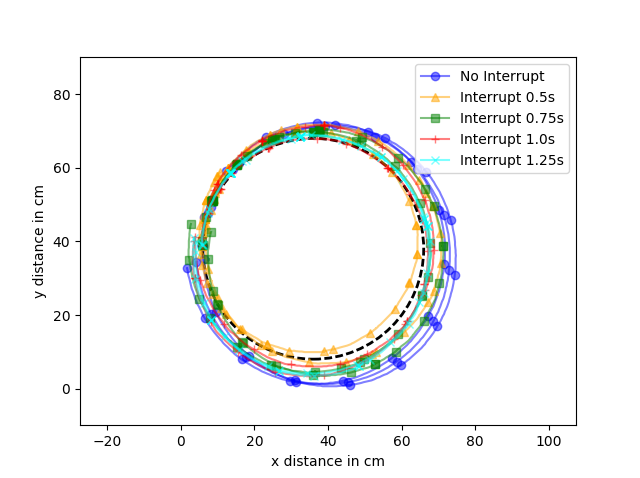
\includegraphics[width=\textwidth]{pics/circle_40.png}
		\caption{Target 40\%}
		\label{fig:circ_exp1}
	\end{subfigure}
	\begin{subfigure}[b]{0.5\textwidth}
		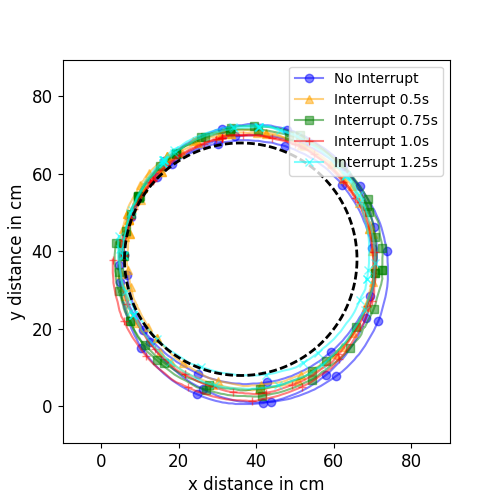
\includegraphics[width=\textwidth]{pics/circle_65.png}
		\caption{Target 65\%}
		\label{fig:circ_exp2}
	\end{subfigure}
	\begin{subfigure}[b]{0.5\textwidth}
		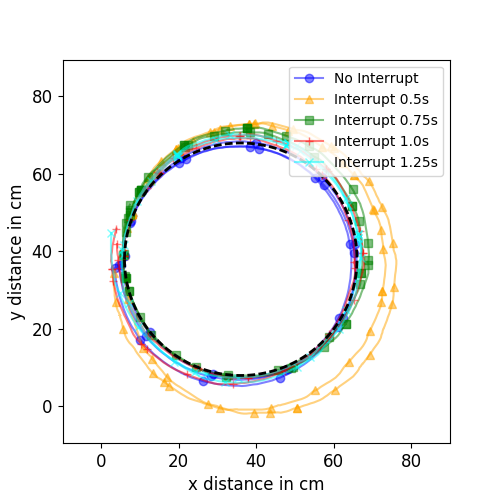
\includegraphics[width=\textwidth]{pics/circle_90.png}
		\caption{Target 90\%}
		\label{fig:circ_exp3}
	\end{subfigure}
	\caption{Circular movements, black dashed circle is the target}
\end{figure}


\subsection{Conclusion}
%Higher speed + more interrupts results in more drift to the left, because of wheel more in the back or weaker motor?
%How the interrupts are distributed over the distance has a influence or how the last interrupt ends up..
%Lower speed and less interrupts results in a higher accuracy??


%For square: Turn\_right speed should be high enough to turn within 0.5 sec


%Observations:
%pwm50 an interrupt every 0.25 sec is uncontrollable
%Lower speed requires longer time between interrupts
%Higher speed + more interrupts results in more drift to the left, because of wheel more in the back or weaker motor?

%Hoe de interrupts uitkomen op de beweging heeft invloed!!

%Lager snelheid en minder interrupts is hogere precisie??


